%%%%%%%%%%%%%%%%%%%%%%%%%%%%%%%%%%%%%%%%%%%%%%%
\chapter{Summary} \label{chap:ending}
%%%%%%%%%%%%%%%%%%%%%%%%%%%%%%%%%%%%%%%%%%%%%%%
\graphicspath{{C:/Users/Kevin/Bachelarbeit/Bachelorarbeit/01_Bachelorarbeit_LaTex/02_Figures/}}
\section{AWGN vs. Rayleigh Comparison}
In this section a short summary between the two simulated channel is given. We will compare the methods and efficiency of both channels and relate it to real world applications. 
\part{title}

\begin{figure}[!htb]
    \centering
    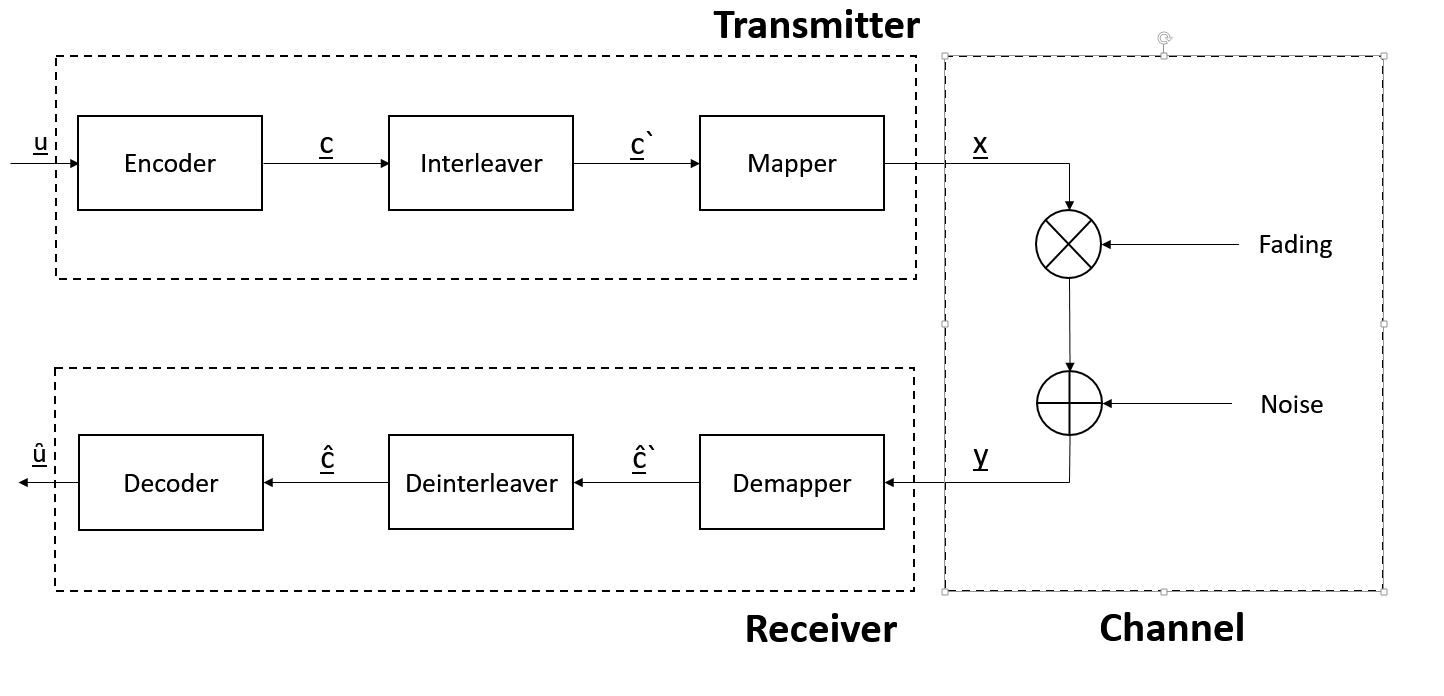
\includegraphics[width=0.8\textwidth]{Channelmodel.PNG}
    \caption{PDF $p_N(N)$ of the number N of times that the head side is up.}
    \label{fig:coin_bino}
\end{figure}



\clearpage
